%\documentclass[slidestop,usepdftitle=false]{beamer}
\documentclass[blue]{beamer}
\usepackage[accumulated]{beamerseminar}
\usepackage{beamertexpower}
%\usepackage[brazil]{babel}
\usepackage[utf8]{inputenc}
\usepackage[portuges]{babel}
\usepackage{stmaryrd} %produto kulkarni-nomizu
\usepackage[normalem]{ulem}%para tachar/riscar o texto \sout{texto}
\usepackage{graphicx}
\usepackage{ragged2e}
\usepackage{graphicx,color}
\usepackage[all]{xy}
%\usepackage[latin1]{inputenc}
\usepackage{amssymb}
\usetheme{Darmstadt}\setbeamercolor{normal text}{}
\graphicspath{{figure/}}
%\usetheme{Hannover}\setbeamercolor{normal text}{bg=green!10}
\title[UFPA]{UM BREVE COMENTÁRIO SOBRE EQUAÇÕES
	DIFERENCIAIS DE PRIMEIRA ORDEM}
\author{Rafael Sergio Sampaio Emidio}
\institute
	{ Trabalho de Conclusão de Curso \\
Instituto de Ciências Exatas e Naturais\\
Orientador: Augusto César dos Reis Costa}
\usetheme{Warsaw}
\newtheorem{proposition}{Proposição}
\newtheorem{cor}{Corolário}
\newtheorem{deff}{Definição}
\newtheorem{thm}{Teorema 1}
\newtheorem{lem}{Lema 1}
\newtheorem{lem2}{Lema 2}
\newtheorem{ex}{Example}
\numberwithin{equation}{section}
%\newtheorem{remark}{Remark}
\newtheorem{remark}{Observação}
\newtheorem{conjec}{Conjectura}
\newcommand{\Gij}[2]{\Gamma_{#1}^{#2}}
\begin{document}
\frame{\titlepage}

\begin{frame}{Resumo}
	\justifying
\hspace{0.2cm} Neste trabalho apresentaremos um breve estudo sobre equações diferenciais ordinárias de primeira ordem. Estudamos alguns métodos analíticos de determinação de soluções e importantes aplicações em determinadas áreas do conhecimento humano; como na biologia, química, física e matemática, envolvendo essas classes de equações e métodos.

\begin{flushleft}
	\justifying
	\textbf{Palavras-chave}: Equações diferenciais de primeira ordem, solução, aplicações.
\end{flushleft}

\end{frame}

\section{Introdução}

\begin{frame}{Introdução}
	\justifying
\hspace{0.2cm} Newton e Leibniz, os criadores do cálculo, foram uns dos primeiros matemáticos que deram início aos estudos das equações diferenciais. Para resolver problemas físicos, era necessário equacionar o fenômeno estudado e através do cálculo de primitivas era possível encontrar a solução do problema. Um dos métodos mais usados era a quadratura, este método consiste em reduzir o problema para obter a solução pelo cálculo de primitivas. Devido ao baixo número de funções que poderiam ser resolvidas por funções elementares, surgiu no século XIX, o uso das séries de funções. Porém, algum tempo depois o método das séries de funções foi sendo usado de uma maneira descuidada, para tentar sanar isso surgiram os teoremas de existência e unicidade, que marcaram o inicío da fase moderna com Poincaré, no final do século XIX. Na evolução dos estudos das equações diferenciais de primeira ordem foram surgindo métodos analíticos para a resolução dessas equações que se originaram de fenômenos físicos, químicos, biológicos, matemáticos, e entre outros.

\end{frame}

\section{Parte teórica}
\begin{frame}{Equações Diferenciais de Primeira Ordem}
	\justifying
\hspace{0.2cm} Uma equação diferencial é uma equação que envolve uma função incógnita e suas derivadas. A forma geral de uma equação diferencial ordinária de primeira ordem é designada por
$$\dfrac{dy}{dt}=f(t,y).$$


\end{frame}

\begin{frame}{Equações Diferenciais Lineares de Primeira Ordem}
	\justifying
\hspace{0.2cm} A forma geral das equações diferenciais ordinárias de primeira ordem é a seguinte
\begin{equation} \label{1}
\dot{x}=p(t)x+q(t),
\end{equation}
onde $\dot{x} = dx/dt$. Precisamos encontrar uma função diferenciável $x: [a,b] \rightarrow \mathbb{R}$ para satisfazer a equação (\ref{1}). Para a solução desta equação, vamos considerar o seguinte problema de valor inicial
\begin{equation} \label{2}
\left\lbrace
\begin{array}{lcl} 
\dot{x} = p(t)x + q(t)\\
x(t_{0})= x_{0}.
\end{array}
\right.
\end{equation}

\hspace{0.2cm} Vamos primeiro determinar a solução geral de (\ref{1}), para depois verificarmos que (\ref{2}) possui apenas uma solução. Consideremos como uma solução de (\ref{1}) uma equação de crescimento exponencial dada por
\begin{equation} \label{3}
\dot{x}=kx(t).
\end{equation}

\end{frame}

\begin{frame}
	\justifying
\hspace{0.2cm} Considerando uma função $x(t)=e^{kt}$ como uma solução de (\ref{3}), os seus múltiplos $ce^{kt}$ também serão soluções de (\ref{3}) e considerando a condição $x(t_{0})=x_{0}$, temos o seguinte problema de valor inicial:
$$\left\lbrace
\begin{array}{lcl}
\dot{x}=kx \\
x(t_{0})=x_{0},
\end{array}
\right.$$
\hspace{0.2cm} Através da condição inicial $x(t_{0})=x_{0}$, o valor da constante $c$ será dado por
$$c=\dfrac{x_{0}}{e^{kt_{0}}}$$
Portanto, obtemos como solução do problema:
$$x(t)=x_{0} e^{k(t-t_{0})},$$
para todo $t \ \epsilon \ \mathbb{R}$.

\hspace{0.2cm} Podemos escrever a equação (\ref{1}) como o seguinte problema de valor inicial com $q(t)\equiv 0$:
\begin{equation} \label{4}
\left\lbrace
\begin{array}{lcl}
\dot{x}= p(t)x \\
x(t_{0})=x_{0}.
\end{array}
\right.
\end{equation}

\end{frame}

\begin{frame}
	\justifying
A equação (\ref{4}) é um problema inicial de valor homogêneo, cuja a solução é dada por
\begin{equation} \label{5}
x(t)=x_{0}e^{\int_{t_{0}}^{t} p(s)\,ds}.
\end{equation}
Com o objetivo de simplificar as expressões, reescrevemos a equação (\ref{5}) da seguinte maneira:
\begin{equation} \label{6}
T(t,t_{0})=e^{\int_{t_{0}}^{t} p(s)\,ds}.
\end{equation}

Temos as seguintes propriedades para a função T:
\begin{equation} \label{7}
\begin{array}{lcl}
T(t_{0},t_{0})= 1, \\
T(t,t_{0}) = T(t_{0},t)^{-1}, \\
T(t,t_{0})T(t_{0},s)=T(t,s).
\end{array}
\end{equation}
\hspace{0.2cm} Voltemos agora, para o problema de valor inicial (\ref{2}), para determinarmos sua solução utilizaremos um fator integrante $\mu(t)$, e multiplicaremos em ambos os lados da equação:
$$\mu(t)(\dot{x}-p(t)x)=\mu(t)q(t).$$
	
\end{frame}

\begin{frame}
	\justifying
Determinaremos $\mu(t)$ igualando o primeiro membro da expressão anterior a derivada do produto de $x$ por $\mu$, logo
$$\mu(\dot{x}-p(t)x) = \dfrac{d}{dt} (\mu x) = \dot{\mu}x + \mu\dot{x}.$$
Então, podemos igualar as seguintes expressões
$$-\mu p(t)x = \dot{\mu}x.$$
Logo, integrando em ambos os lados, obtemos
$$ln \mu = - \int p(s) \, ds.$$
\hspace{0.2cm} Logo, $\mu (t)$ será dado por:
$$\mu (t) = e^{- \int_{t_{0}}^{t} p(s) \, ds} = e^{\int_{t}^{t_{0}} p(s) \, ds} = T(t_{0},t).$$
	
\end{frame}

\begin{frame}
	\justifying
	Então temos de $\dfrac{d}{dt} (\mu x) = \mu(t)q(t)$:
	$$\dfrac{d}{dt}(T(t_{0},t) x(t)) = T(t_{0},t)q(t),$$
	integrando em ambos os lados de $t_{0}$ a $t$:
	$$T(t_{0},t)x(t)-x(t_{0}) = \int_{t_{0}}^{t} T(t_{0},s)q(s) \, ds.$$
	\hspace{0.2cm} Portanto, podemos obter a solução do problema de valor inicial (\ref{2}) e utilizando as propriedades (\ref{7}), multiplicamos a última expressão por $T(t,t_{0})$ e vamos obter:
	\begin{equation} \label{8}
	x(t) = T(t,t_{0})x_{0} + \int_{t_{0}}^{t} T(t,s)q(s) \, ds,
	\end{equation}
	a equação (\ref{8}) é chamada de fórmula de variação de constantes, fórmula esta que pode ser escrita como solução do problema de valor inicial (\ref{2}).
	
	
\end{frame}

\begin{frame}
	\justifying
\hspace{0.2cm} Em particular, se o coeficiente $p(t)$ for igual a uma constante $k$, temos
$$T(t,t_0) = e^{k(t-t_0)}.$$
Então temos o seguinte problema de valor inicial
$$\left\lbrace
\begin{array}{lcl} 
\dot{x} = kx + q(t)\\
x(t_{0})= x_{0},
\end{array}
\right.$$
e pela fórmula de variação de constantes, dada na equação (\ref{8}), obtemos
$$x(t)=e^{k(t-t_0)}x_0 + \int_{t_{0}}^{t} e^{k(t-s)}q(s)ds.$$
\hspace{0.2cm} Se existe um ponto $a$ associado a uma função $x_1(t)$ e um ponto $b$ associado a uma função $x_2(t)$, podemos verificar que essas funções são soluções do problema de valor inicial (\ref{1}) da seguinte maneira: 
$$x_1(t) = ae^{\int_{t_0}^{t} p(s) \,ds},$$
$$x_2(t) = be^{\int_{t_0}^{t} p(s) \,ds}.$$
	
\end{frame}

\begin{frame}
	\justifying
Logo,
$$x_1(t)- x_2(t) = (a-b)e^{\int_{t_0}^{t} p(s) \,ds}$$
$$x(t) = x_0e^{\int_{t_0}^{t} p(s) \,ds},$$
então podemos afirmar que $x(t) = x_1(t) - x_2(t)$ é uma solução do problema de valor inicial (\ref{4}), onde $x_0 = a - b$. Logo, todas as soluções de (\ref{1}) são obtidas somando uma solução particular com a solução geral da equação homogênea associada em (\ref{4}). Logo, podemos dizer que o termo da fórmula da variação de constantes 
$$\int_{t_{0}}^{t} e^{k(t-s)}q(s)ds$$
é uma solução particular de (\ref{1}). 
	
\end{frame}

\begin{frame}{Equações Separáveis}
\justifying
\hspace{0.2cm} Uma equação diferencial da forma
\begin{equation} \label{10}
y' = \dfrac{f(x)}{g(y)},
\end{equation}
é chamada de equação separável, onde $g(y) \neq 0$ e $y' = dy / dx$. Consideramos $f$ e $g$ funções contínuas em intervalos abertos reais, tal que $f: (a,b) \rightarrow \ \mathbb{R}$ e $g: (c,d) \rightarrow \ \mathbb{R}$. Logo escrevemos (\ref{10}) da forma
\begin{equation} \label{11}
g(y)y' = f(x).
\end{equation}
\hspace{0.2cm} Considerando uma função $y: (\alpha, \beta) \rightarrow \ \mathbb{R}$ de classe $C^{1}$ uma solução para (\ref{10}) e $G$ uma primitiva de $g$, onde $G' = g$, teremos a partir de (\ref{11}):
$$g(y) \dfrac{dy}{dx} = f(x)$$

\end{frame}

\begin{frame}
	\justifying
então obtemos
\begin{equation} \label{12}
G(y(x)) = F(x) + C,
\end{equation}
onde $F$ é uma primitiva de $f$.
\hspace{0.2cm} Dado um ponto $x_0 \ \epsilon \ (\alpha, \beta)$, então temos uma condição inicial dada por $y(x_0) = y_0$, onde $y_0 \epsilon \ y(\alpha, \beta)$. Logo a constante $C$ será dada determinada por
$$C = G(y_0) - F(x_0),$$
substituindo $C$ na expressão (\ref{12}), vamos obter
$$G(y(x)) - G(y_0) = F(x) - F(x_0).$$
Como $G$ é uma primitiva de $g$ e $F$ é uma primitiva de $f$, podemos escrever a última expressão como
\begin{equation} \label{13}
\int_{y_0}^{y(x)} g(y) \, dy =  \int_{x_0}^{x} f(x) \, dx.
\end{equation}
	
\end{frame}

\begin{frame}
	\justifying
\hspace{0.2cm} O que mostramos acima foi que dada uma solução de (\ref{10}), esta solução irá satisfazer a expressão (\ref{12}). Podemos concluir que dada uma relação $G(y) = F(x) + C$ e um ponto $(x_0, y_0)$ que satisfaz essa relação, onde $G'(y_0) = g(y_0) \neq 0$, dado também um intervalo aberto $(\alpha, \beta)$ contendo $x_0$ e uma função de classe $C^{1}$, através do Teorema das funções implícitas podemos garantir que esse intervalo existe e que satifaz a relação (\ref{12}), logo trata-se de uma solução de (\ref{1}).

\begin{flushleft}
	\justifying
	\textbf{Exemplo 1}: Resolva a equação $y' = \dfrac{x}{y}.$ 
	\newline
	\underline{Resolução}: Como $yy' = x$, teremos como solução geral $y^{2} = x^{2} + C$. Se considerarmos um problema de valor inicial com a condição $y(3) = 2$, obtemos $C = - 5$, logo a solução é dada por \end{flushleft}
$$y(x) = +\sqrt{x^2 - 5}, \ x > \sqrt{5}.$$
	
\end{frame}

%\begin{frame}
%\justifying
%\begin{flushleft}
%	\textbf{Definição 2.1}: Uma equação da forma \end{flushleft}
%\begin{equation} \label{14}
%\dot{x} = f(x)
%\end{equation}
%é chamada de equação autônoma, pois a função $f$ depende apenas de $x$ e não da variável independente $t$. 
%
%\begin{flushright}
%	\justifying
%	\textbf{Definição 2.2}: Se $\bar{x}$ é um zero da função, ou seja, $f(\bar{x}) = 0$, logo $x(t) \equiv \bar{x}$ é uma solução de (\ref{14}). Sendo assim, $x(t)$ é chamada de solução equilíbrio ou estacionária e o ponto $\bar{x}$ é chamado de ponto de equilíbrio ou singularidade.\end{flushright} 
%
%\begin{flushleft}
%	\justifying
%	\textbf{Teorema 2.1}: Se $\bar{x}$ é um ponto de equilíbrio e $f(\bar{x})$ é uma solução de (\ref{14}), $\bar{x}$ é assintoticamente estável se $f'(\bar{x}) < 0$ e $\bar{x}$ é assintoticamente instável quando $f'(\bar{x}) > 0$. \end{flushleft}
%
%\end{frame}

\begin{frame}
	\justifying
\begin{flushleft}
	\justifying
	\textbf{Teorema}: Seja $\Omega$ um intervalo aberto no plano $(x,y)$, neste intervalo está definido a função contínua $f:\Omega \rightarrow \mathbb{R}$. Supondo que a derivada parcial em relação à $y$, dada por $f_y:\Omega \rightarrow \mathbb{R}$ também seja contínua, temos para cada ponto $(x_0,y_0)$ em $\Omega$ um intervalo aberto $I$ que contém $x_0$, uma única função diferenciável $\phi: I \rightarrow \mathbb{R}$, onde $(x,\phi(x)) \ \epsilon \ \Omega$ para todo $x \ \epsilon \ I$. Logo, $\phi$ será a solução do problema de valor inicial dado por
\end{flushleft}
$$\left\lbrace
\begin{array}{lcl} 
y' = f(x,y)\\
y(x_0) = y_0.
\end{array}
\right.$$
	
\end{frame}

\section{Aplicações}
\begin{frame}{Dinâmica de uma População e Noções de Estabilidade}
\justifying

%\hspace{0.2cm} Nesta sessão veremos os conceitos de estabilidade e instabilidade através de alguns modelos  criados para análise da variação de uma população com o tempo. Cada modelo leva em conta a influência de vários fenômenos biológicos e sociológicos na evolução da população, e cada modelo possui uma taxa de crescimento da população $p(t)$, onde $t$ é o tempo, taxa essa definida por $\dot{p}(t)/ p(t)$.

\begin{flushleft}
	$\bullet$ O Modelo Malthusiano
\end{flushleft}
\hspace{0.2cm} Este modelo basicamente assume que a taxa de crescimento de uma população é dado por uma constante $\lambda$, então a equação que rege o crescimento dessa população é dado
\begin{equation} \label{17} 
\dot{p} = \lambda p.
\end{equation}

\end{frame}

\begin{frame}
\justifying
\hspace{0.2cm} Considerando $p_0$ como população inicial, temos como solução geral do problema de valor inicial homogêneo (\ref{17}):
$$p(t)= p_0 e^{\lambda(t-t_0)},$$
e com a condição inicial $p(t_0) = p_0$, a solução para (\ref{17}) é dada por
$$p(t) = p(t_0)e^{\lambda(t-t_0)},$$
onde esta solução apresenta um crescimento exponencial se $\lambda > 0$, porém não é possível que este crescimento se mantenha para sempre. Um modelo desta natureza pode descrever o crescimento populacional de micro-organismos que se reproduzem por mitose. 

\end{frame}

\begin{frame}{}
	\justifying
	\begin{flushleft}
		$\bullet$ O Modelo de Verhulst - A Logística
	\end{flushleft}
	
	\hspace{0.2cm} Neste modelo proposto por Verhulst em 1834, constante $\lambda$ é a taxa de crescimento da população, dado pela diferença entre a taxa de natalidade e a taxa de mortalidade, ou seja: $\lambda = \lambda_n - \lambda_m$. Verhulst propôs um modelo em que a taxa de crescimento decresce linearmente com a população, modelo este dado por: $\lambda = a - bp$, onde $a$ e $b$ são constantes positivas. Este modelo é dado por
	\begin{equation} \label{18}
	\dot{p} = (a-bp)p.
	\end{equation} \\
	\hspace{0.2cm} Podemos observar que ainda não é um modelo ideal, pois não leva em conta que a taxa de produção de novos seres da espécie humana, depende da idade dos pais. 
	
\end{frame}

\begin{frame}
\justifying
\hspace{0.2cm} Considerando $p(t_0) = p_0$ como condição inicial, a solução para (\ref{18}) será dada por:
\begin{equation} \label{20}
p(t) = \dfrac{a p_0}{p_0 b + (a - bp_0)e^{-a(t-t_0)}}.
\end{equation}

\begin{flushright}
	\justifying
	\textbf{Análise da solução}: A solução do modelo proposto por Verhulst, forma o gráfico da chamada curva logística. Onde este gráfico forma uma curva em forma de S entre as retas $p = 0$ e $p = a/b$ (soluções de (\ref{18})). Em $p = a/2b$ existe um ponto de inflexão pois $a/2b$ é uma solução para $\ddot{p}$. Esta curva é formada para o caso $0 <\ p_0 <\ a/b$, para $p_0 >\ a/b$ a curva descresce exponencialmente para $a/b$. \end{flushright}

\end{frame}

%\begin{frame}
%	\begin{flushright}
%		\justifying
%		\textbf{Análise da solução}: Analisando (\ref{18}), podemos ver $p(t) = 0$, $p(t) = a/b \equiv p_\infty$ são suas soluções. A notação $p_\infty$ é justificada da seguinte maneira: se em (\ref{20}) $t \rightarrow \infty$, logo $p(t) \rightarrow p_\infty$. Então de (\ref{20}) obtemos que $p_\infty = a/b$, esta solução é chamada de população limite e será o valor assintótico para uma população inicial, tal que $p_0 >\ 0$. Podemos analisar dois casos: o primeiro se $p_0 > p_\infty$ e o segundo se $0 < p_0 < p_\infty$. No primeiro caso, p(t) descresce exponencialmente tendendo para $p_\infty$. No segundo caso, a população irá crescer e também tenderá a $p_\infty$, onde o gráfico de $p(t)$ será uma curva em forma de S entre as retas $p =0$ e $p = p_\infty$, esta curva é chamada de logística. Pois derivando (\ref{18}), obtemos:\end{flushright}
%	$$\ddot{p} = (a - 2bp)\dot{p}.$$
%	
%\end{frame}

%\begin{frame}
%	\hspace{0.2cm} Podemos concluir que a curva logística tem um ponto de inflexão quando $p(t) = \dfrac{a}{2b}$, pois
%	$$\ddot{p} = (a - 2b\dfrac{a}{2b})\dot{p} = 0,$$ 
%	significa que a população cresce com derivada positiva e em seguida o crescimento se torna mais lento, isto ocorre até a função atingir o valor $p_\infty/2$.
%	
%\end{frame}

\begin{frame}{}
		\begin{figure}[ht!]
		\centering
		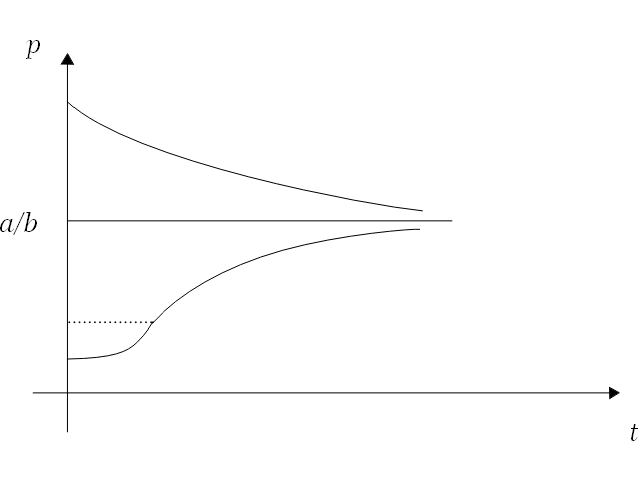
\includegraphics[width=10cm]{Figura1}
		\caption{Curva logística}
	\end{figure}
\end{frame}

\begin{frame}{Resfriamento de um Corpo}
	\justifying
	
	\hspace{0.2cm} Podemos analisar o fenômeno da variação de temperatura em um corpo por perda de calor para o meio ambiente através do seguinte modelo:
	\begin{equation} \label{21}
	\dfrac{dT}{dt} = -k(T - T_a),
	\end{equation}
	onde $dT/dt$ é o fluxo de calor, $T$ é a temperatura do corpo dependente do tempo $t$, $T_a$ é a temperatura do meio ambiente, $k$ é uma constante positiva determinada pelas propriedades físicas do corpo. Na situação dada, o calor flui da fonte quente para fonte fria, então se $T > T_a$, a temperatura $T$ descresce e o corpo se resfria, portanto isto justifica o sinal negativo em (\ref{21}). Agora, se $T < T_a$, a temperatura $T$ cresce e o corpo irá se aquecer. O modelo apresentado acima é chamada Lei de Resfriamento de Newton, Newton elaborou este modelo estudando uma bola de metal aquecida.
	
\end{frame}

\begin{frame}
	\justifying
\hspace{0.2cm} Considerando a condição inicial de temperatura $T(0) = T_0$, temos o seguinte problema de valor inicial:
$$\left\lbrace
\begin{array}{lcl} 
\dfrac{dT}{dt} = -k(T - T_a) \\
\\
T(0) = T_0.
\end{array}
\right.$$
Através do métodos da sessão 2.1, a solução do problema é dada por
$$T - T_a = e^{-kt + C},$$
usando a condição inicial $T(0) = T_0$,
$$e^{C} = T_0 - T_a.$$
Logo, obtemos a solução do problema:
\begin{equation} \label{22}
T = (T_0 - T_a)e^{-kt} + T_a.
\end{equation}
	
\end{frame}

\begin{frame}
\begin{flushleft}
	\justifying
	\textbf{Análise da solução}: Na expressão (\ref{21}), podemos ver que $T(t)$ descrece monotonicamente com $t$ quando $T > T_a$, $T(t)$ irá crescer monotonicamente quando $T < T_a$ e quando for $T(t)$ for constante teremos $T = T_a$. Na expressão (\ref{22}) temos a mesma conclusão, pois $T(t)$ tende monotonicamente para $T_a$ quando $t \rightarrow +\infty$. Portanto, a temperatura $T_a$ é chamada Temperatura de Equilíbrio.\end{flushleft}
	
\end{frame}

\begin{frame}{Diluição de Soluções}
\justifying
\hspace{0.2cm} Um reservatório com capacidade de $V$ litros de água pura, recebe uma solução de água salgada que contém $c$ kg de sal por litro de solução, a uma vazão de a litros/segundo de forma constante. Portanto, seja $x(t)$ a quantidade de sal em kg no reservatório em função do tempo $t$, a concentração de sal na solução é dada por $x/V$ $kg/l$. Então podemos descrever esta situação através da seguinte equação diferencial:
\begin{equation} \label{26}
\dfrac{dx}{dt} = ac - a\dfrac{x}{V},
\end{equation}
e considerando a condição $x(0) = 0$, temos o seguinte problema de valor inicial:
$$\left\lbrace
\begin{array}{lcl} 
\dfrac{dx}{dt} + a\dfrac{x}{V} = ac \\
\\
x(0) = 0.
\end{array}
\right.$$
\end{frame}

\begin{frame}
	\hspace{0.2cm} Para encontrarmos a solução do problema, precisamos determinar o fator integrante $\mu (t) = e^{\int{a(t) dt}}$, onde $a(t) = \dfrac{a}{V}$, logo
	$$\mu (t) = e^{\frac{at}{V}}.$$
	Então, multiplicando todos os membros da equação (\ref{26}), por $\mu (t)$, obtemos
	$$(\mu x) \dfrac{d}{dt} = ac e^{\frac{at}{V}}$$
	$$x = cV + k e^{-\frac{at}{V}}.$$
	Para determinar $k$, utilizamos a condição inicial $x(0) = 0$, logo
	$$k = - cV.$$
	Portanto a solução do problema será dada por:
	\begin{equation}\label{27}
	x(t) = cV(1 - e^{-\frac{at}{v}})
	\end{equation}
		
\end{frame}

\begin{frame}
\begin{flushleft}
	\justifying
	\textbf{Análise da solução}: Podemos notar que quando $t \rightarrow \infty$, a concentração de sal dada por $x(t)/V$ tende para $c$, assim como em resfriamento de um corpo em que a solução nos dava uma temperatura de equilíbrio, no caso de diluição das soluções podemos encontrar o equilíbrio entre a solução salina injetada e a solução no reservatório, pois em ambos os casos a matemática é a mesma. \end{flushleft}

\end{frame}

%\begin{frame}{Por que uma corda enrolada em um poste sustenta um barco?}
%\justifying
%\hspace{0.2cm} Imaginemos uma corda presa a uma superfície cilíndrica vertical com coeficiente de atrito estático $\mu$. O contato da corda com a superficíe gera um setor circular $AB$ com ângulo $\alpha < 180$°. Existe uma força $T_0$ aplicada em uma das extremidades e na outra extremidade uma força $T_1$, onde essas forças estão em equilíbrio.
%
%\end{frame}
%
%\begin{frame}
%\begin{figure}[ht!]
%	\centering
%	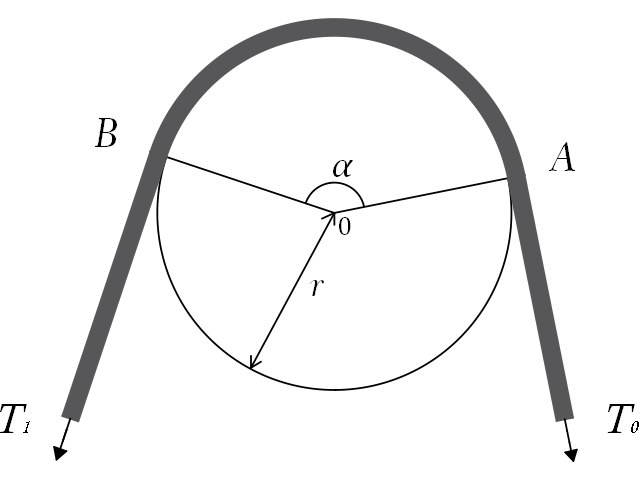
\includegraphics[width=10cm]{Figura2}
%	\caption{Corda amarrada a uma superfície cilíndrica de forma vertical}
%\end{figure}
%\end{frame}
%
%\begin{frame}{}
%\begin{figure}[ht!]
%	\centering
%	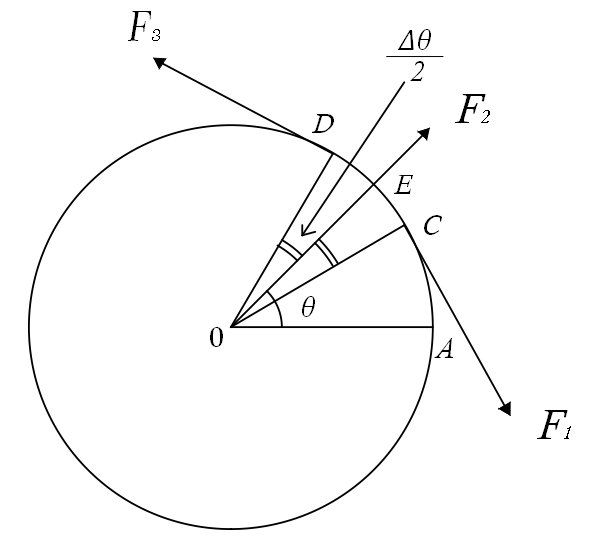
\includegraphics[width=8cm]{Figura3}
%	\caption{Decomposição das forças que atuam na corda}
%\end{figure}
%\end{frame}
%
%\begin{frame}
%	\justifying
%	\hspace{0.2cm} Sabendo que $T(\theta)$ é a tensão no ponto da corda que corresponde ao ângulo $\theta$ a partir do segmento $0A$ no sentindo anti-horário, fazemos as seguintes análises: \\\
%	$F_1$ é a tensão da corda no ponto C, o que implica
%	$$\vert F_1 \vert = T\left(\theta - \dfrac{\Delta\theta}{2}\right).$$
%	
%\end{frame}
%
%\begin{frame}
%\justifying
%$F_2$ é a soma da tensão no ponto D com a força de atrito a partir de $F_3$, logo
%$$\vert F_2 \vert = T\left(\theta + \dfrac{\Delta\theta}{2}\right) + \mu \vert F_3 \vert.$$
%$F_3$ será a reação total da superficíe ao longo do arco $CD$, dado por
%$$\vert F_3 \vert = N(\theta) r \Delta\theta,$$
%onde $N(\theta)$ é a reação da superfície sobre a corda e $r\Delta\theta$ é comprimento do arco $CD$.
%
%\hspace{0.2cm} Analisando as forças $F_2$ e $F_3$, podemos notar que a força de atrito é dada por $\mu N(\theta) r \Delta\theta$, onde sabemos pela análise da força $F_3$ que $N(\theta) r \Delta\theta$ é a reação total da superfície ao longo do arco $CD$ e que possui comprimento $r\Delta\theta$. Pelo fato do arco $CD$ estar em equilíbrio, temos que $F_1 + F_2 + F_3 = 0$, logo projetando a equação sobre a direção $F_3$.
%\end{frame}
%
%\begin{frame}{}
%\begin{figure}[ht!]
%	\centering
%	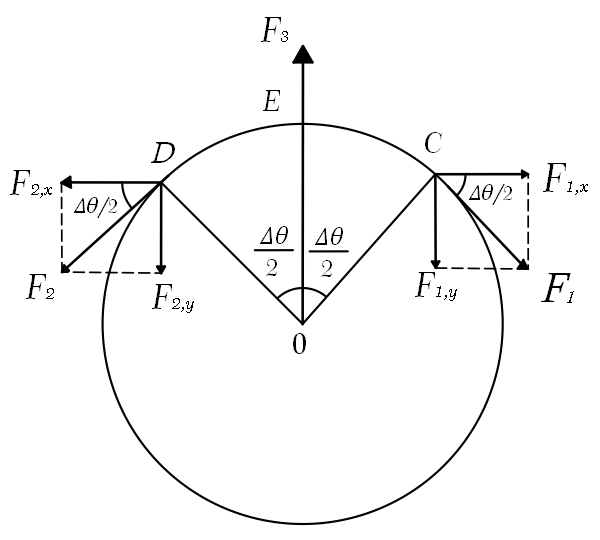
\includegraphics[width=8cm]{Figura4}
%	\caption{Diagrama de forças}
%\end{figure}
%\end{frame}
%
%\begin{frame}
%	\justifying
%	\hspace{0.2cm} Analisando o diagrama de forças, temos as seguintes equações:
%	$$- F_{1,y} - F_{2,y} + F_3 = 0,$$
%	$F_{1,y}$ será dado por $T \left(\theta - \dfrac{\Delta\theta}{2}\right) sen \dfrac{\Delta\theta}{2},$ \\\
%	$F_{2,y}$ será dado por $T \left(\theta + \dfrac{\Delta\theta}{2}\right) sen \dfrac{\Delta\theta}{2} + \mu N(\theta) r \Delta\theta sen \dfrac{\Delta\theta}{2}.$ 
%	
%\end{frame}
%
%\begin{frame}
%	\justifying
%	\hspace{0.2cm} Portanto, temos a seguinte expressão:
%	\begin{eqnarray} \label{28}
%	&N(\theta) r \Delta\theta - T \left(\theta - \dfrac{\Delta\theta}{2}\right) sen \dfrac{\Delta\theta}{2} - T \left(\theta + \dfrac{\Delta\theta}{2}\right) sen \dfrac{\Delta\theta}{2} \nonumber \\
%	& - \mu N(\theta) r \Delta\theta sen \dfrac{\Delta\theta}{2} = 0.
%	\end{eqnarray}
%	
%	\hspace{0.2cm} Na demonstração acima analisamos as forças na direção do eixo y, agora na direção do eixo x, temos
%	$$F_{1,x} - F_{2,x} = 0,$$
%	$F_{1,x}$ será dado por $T \left(\theta - \dfrac{\Delta\theta}{2}\right) cos \dfrac{\Delta\theta}{2},$ \\\
%	$F_{2,x}$ será dado por $T \left(\theta + \dfrac{\Delta\theta}{2}\right) cos \dfrac{\Delta\theta}{2} + \mu N(\theta) r \Delta\theta cos \dfrac{\Delta\theta}{2}.$
%	
%	\hspace{0.2cm} Portanto, obtemos a seguinte expressão:
%	\begin{equation} \label{29}
%	T \left(\theta - \dfrac{\Delta\theta}{2}\right) cos \dfrac{\Delta\theta}{2} - T \left(\theta + \dfrac{\Delta\theta}{2}\right) cos \dfrac{\Delta\theta}{2} - \mu N(\theta) r \Delta\theta cos \dfrac{\Delta\theta}{2} = 0.
%	\end{equation}
%	
%\end{frame}
%
%\begin{frame}
%\justifying
%\hspace{0.2cm} Dividindo as equações (\ref{28}) e (\ref{29}) por $\Delta\theta$ e aplicando o limite quando $\Delta\theta \rightarrow 0$, obtemos duas equações dadas por:
%\begin{equation} \label{30}
%rN(\theta) - T(\theta) = 0,
%\end{equation}
%\begin{equation} \label{31}
%\dfrac{dT}{d\theta} (\theta) + \mu r N(\theta) = 0.
%\end{equation}
%Isolando $N(\theta)$ em (\ref{30}) e substituindo em (\ref{31}), obtemos
%$$\dfrac{dT}{d\theta} + \mu T = 0.$$
%
%\hspace{0.2cm} Considerando a condição $T(0) = T_0$, temos o seguinte problema de valor inicial:
%$$\left\lbrace
%\begin{array}{lcl} 
%\dfrac{dT}{d\theta} + \mu T = 0 \\
%\\
%T(0) = T_0.
%\end{array}
%\right.$$
%
%\end{frame}
%
%\begin{frame}
%\justifying
%Resolvendo o problema, temos 
%$$ln T = -\mu\theta + c$$
%$$T = e^{c} \cdot e^{-\mu\theta},$$
%considerando a condição inicial $T(0) = T_0$, obtemos
%$$e^{c} = T_0.$$
%Então a solução do problema é dada por
%$$T(\theta) = T_0 e^{-\mu\theta}.$$
%
%\begin{flushleft}
%	\justifying
%	\textbf{Análise da solução}: Podemos concluir que a força para a corda sustentar um barco enrolada num poste gerando um setor de ângulo $\alpha$ é dada por $T_1 = T_0 e^{-\mu\alpha}$. Então podemos notar que quanto menor for o ângulo $\alpha$, menor será $T_1$, ou seja, menor será a força necessária para aplicar na outra extremidade como mostra figura 2. Então, concluimos que quanto mais voltas a corda fizer no poste, a força $T_1$ será tão pequena que apenas o peso da corda jogada sobre o solo é suficiente para manter o equilíbrio.
%\end{flushleft}
%
%
%\end{frame}

\begin{frame}{A Tractriz}
	\justifying
	\hspace{0.2cm} Uma partícula $Q$ de massa $m$, será arrastada ao longo de uma corda $QP$, essa corda é mantida de forma bem esticada e sua extremidade $P$ está sobre o eixo $x$, então a tractriz é formada ao longo da curva descrita pela partícula $Q$ como é mostrado na figura 6.
	\begin{figure}[ht!]
		\centering
		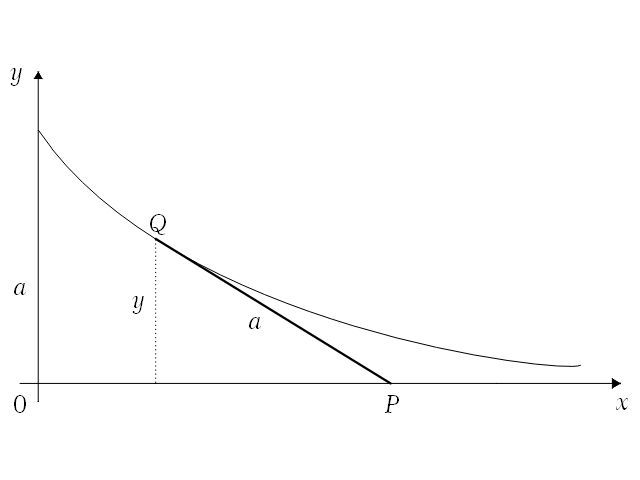
\includegraphics[width=8cm]{Figura6}
	\end{figure}
	
\end{frame}

\begin{frame}
	\justifying
	\hspace{0.2cm} Considerando as coordenadas $Q(x,y)$, $P(x_a,0)$ e $R(x,0)$, temos a seguinte relação pelo teorema de Pitágoras: 
$$QP^{2} = QR^{2} + RP^{2}$$
$$a^2 = y^2 + (x - x_a)^{2},$$
isolando o termo $x - x_a$, obtemos
$$x - x_a = \pm \sqrt{a^2 - y^2}.$$
Para o problema vamos considerar $- \sqrt{a^2 - y^2}$. Então, lembrando da equação da reta que passa por um ponto, temos 
$$y - y(x_a) = y' \cdot (x - x_a),$$
sabendo que $y(x_a) = 0$, teremos a seguinte equação diferencial:
\begin{equation} \label{37}
y' = - \dfrac{y}{\sqrt{a^{2} - y^{2}}}.
\end{equation}
\end{frame}

\begin{frame}
	\justifying
	\hspace{0.2cm} Sabendo que $y' = dx/dy$, podemos rescreever a expressão (\ref{37}) da seguinte maneira: 
	$$-dx = \dfrac{\sqrt{a^{2} - y^{2}}}{y} dy,$$ 
	uma primitiva de $\sqrt{a^{2} - y^{2}}/y$, é dada por
	$$ - x + c = a \hspace{0.1cm} ln \left(\dfrac{a - \sqrt{a^2 - y^2}}{y}\right) + \sqrt{a^2 - y^2}.$$
	\hspace{0.2cm} Considerando o problema de valor inicial com a condição $y(0) = a$, vamos obter que $c = 0$. Portanto a solução da equação diferencial (\ref{37}) será dada por
	$$x = - a \hspace{0.1cm} ln \left(\dfrac{a - \sqrt{a^2 - y^2}}{y}\right) - \sqrt{a^2 - y^2},$$
	onde esta solução é a equação da tractriz $x(y)$, explicitada de maneira que $y$ é a variável independente e $x$ sendo a variável dependente.
	
\end{frame}

\begin{frame}{As Curvas de Perseguição}
	\justifying
\hspace{0.2cm} Vamos imaginar que um gato persegue um rato no plano $(x,y)$. O rato estava comendo queijo na origem e o gato localizado no ponto $G = (a,0)$, o gato faminto parte em direção ao rato e o rato por sua vez, foge do gato correndo ao longo do eixo $y$ no sentido positivo com uma velocidade constante $\nu$. O gato ao correr em direção ao rato com uma velocidade constante $\omega$, forma uma curva como podemos ver na figura 12, e o problema desta sessão consiste em determinar a curva descrita pelo gato nos parâmetros $a, \nu$ e $\omega$. 

\end{frame}

\begin{frame}{}
	\begin{figure}[ht!]
	\centering
	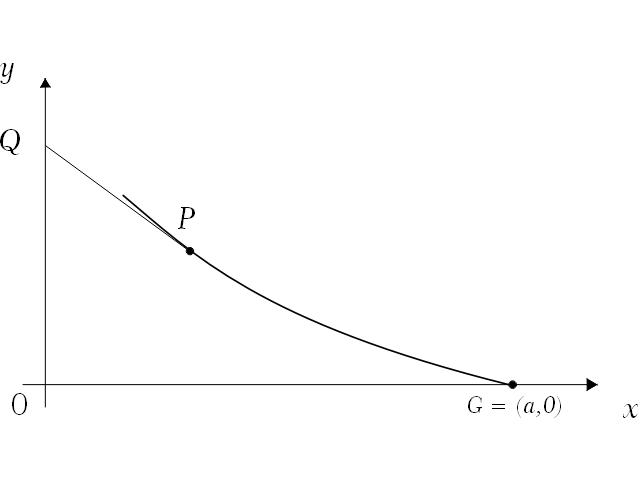
\includegraphics[width=10cm]{Figura12}
	\caption{Curva de perseguição.}
\end{figure}
\end{frame}

\begin{frame}
\justifying
\hspace{0.2cm} Considerando que após um tempo $t$, o gato estará em um ponto $P = (x,y)$ e como o deslocamento do rato se dá ao longo do eixo $y$, logo a sua segunda coordenada será dada por esse deslocamento, então ele estará no ponto $Q = (0,\nu t)$ c. Olhando agora para o deslocamento do gato, podemos calcular o seu deslocamento $L$ através do comprimento de arco $PG$ que vai de $a$ até $x$, então teremos 
$$L = \int_x^a \sqrt{1 + |y'(x)|^2} dx,$$
sabendo que o deslocamento $L$ é dado por $t \omega$, o tempo que o gato levou para chegar até o ponto $P$ será dado por
\begin{equation} \label{50}
t = \dfrac{1}{\omega} \int_x^a \sqrt{1 + |y'(x)|^2} dx.
\end{equation}

\hspace{0.2cm} Agora, considerando o ponto $P$ de coordenadas arbitrárias $(x,y)$ temos pela geometria da figura:
$$y' = \dfrac{\bar{OQ} - y}{0 - x},$$

\end{frame}

\begin{frame}
	\justifying
	logo 
	$$\bar{OQ} = y - y'x,$$
	e como $\bar{OQ} = \nu t$,
	\begin{equation} \label{51}
	\nu t = y - y'x.
	\end{equation}
	Logo, de (\ref{50}) e (\ref{51}), temos a expressão
	$$\dfrac{\nu}{\omega} \int_x^a \sqrt{1 + |y'(x)|^2} dx = y - y'x,$$
	derivando a expressão acima em relação a variável $x$, obtemos
	\begin{equation} \label{52}
	c\sqrt{1 + |y'(x)|^2} = xy'',
	\end{equation}
	onde $c = \nu / \omega$. Introduzindo a variável $p = y'$, teremos a seguinte expressão
	\begin{equation} \label{53}
	c\sqrt{1 + p^2} = xp'.
	\end{equation}
		
\end{frame}

\begin{frame}
\justifying
\hspace{0.2cm} Sabendo que $p' = dp/dx$, temos o seguinte problema de valor inicial:
$$\left\lbrace
\begin{array}{lcl} 
\dfrac{c}{x} dx = \dfrac{1}{\sqrt{1 + p^2}} dp \\
\\
p(a) = 0.
\end{array}
\right.$$
Uma primitiva de $1/\sqrt{1 +p^2}$ é dada por
$$-ln(\sqrt{p^2 + 1} - p),$$
logo a solução geral do problema de valor inicial será dada por
$$c \cdot lnx + k = - ln(\sqrt{p^2 + 1} - 1).$$
Utilizando a condição inicial $p(a) = 0$, vamos obter
$$k = -c \cdot lna.$$
	
\end{frame}

\begin{frame}
	\justifying
	\hspace{0.2cm} Então vamos obter da solução de (\ref{53}):
	$$c \cdot lna - c \cdot lnx = ln(\sqrt{p^2 + 1} - 1)$$ 
	\begin{equation} \label{54}
	\sqrt{p^2 + 1} - p = \left(\dfrac{a}{x}\right)^c.
	\end{equation}
	Da expressão (\ref{54}), isolando a variável $p$, obtemos
	$$p = \dfrac{1}{2} \left[\left(\dfrac{x}{a}\right)^c - \left(\dfrac{a}{x}\right)^c \right].$$
	Sabendo que $p = y' = dy/dx$, temos o seguinte problema de valor inicial:
	$$\left\lbrace
	\begin{array}{lcl} 
	y' = \dfrac{1}{2} \left[\left(\dfrac{x}{a}\right)^c - \left(\dfrac{a}{x}\right)^c \right] \\
	\\
	y(a) = 0.
	\end{array}
	\right.$$
	\hspace{0.2cm} Para $c\neq1$, vamos obter como solução geral do problema:
	$$y = \dfrac{a}{2} \left[\dfrac{1}{c+1} \left(\dfrac{x}{a}\right)^{c+1} + \dfrac{1}{c-1} \left(\dfrac{a}{x}\right)^{c-1} \right] + k.$$
		
\end{frame}

\begin{frame}
	\justifying
\hspace{0.2cm} Utilizando a condição inicial $y(a) = 0$,
$$k = - \dfrac{ac}{c^2 - 1}.$$
Portanto, a solução do problema de valor inicial será dada por
\begin{equation} \label{55}
y(x) = \dfrac{a}{2} \left[\dfrac{1}{c+1} \left(\dfrac{x}{a}\right)^{c+1} + \dfrac{1}{c-1} \left(\dfrac{a}{x}\right)^{c-1} \right] - \dfrac{ac}{c^2 - 1}.
\end{equation}

\begin{flushleft}
	\justifying
	\textbf{Análise da solução}: Se considerarmos $c\geq1$, consequentemente a velocidade do rato seria maior que a do gato, ou seja, $\nu\geq\omega$. Porém, se analisarmos o caso para $c <\ 1$, vamos ter que a velocidade do gato será a maior, ou seja, $\nu <\ \omega$. Podemos determinar o instante e o ponto da coordenada sobre o eixo $y$ onde o encontro entre os dois aconteceria. \end{flushleft}
	
\end{frame}

\begin{frame}
	\justifying
\hspace{0.2cm} Para determinar o instante, utilizaremos a equação (\ref{55}), para $y(0) = \nu t$, onde $\nu t$ representa o deslocamento do rato. Logo obtemos que o instante que o gato encontra o rato é dado por
$$t = \dfrac{a\omega}{\omega^2 - \nu^2}.$$

\hspace{0.2cm} Já o ponto de encontro entre os dois, também pode ser encontrado pela expressão (\ref{55}), agora considerando a condição $y(0) = E$, onde $E$ será o ponto de encontro. Logo temos que o ponto da ordenada sobre o eixo $y$ onde o gato encontra o rato, é dado por
$$E = \dfrac{a\nu\omega}{\omega^2 - \nu^2}.$$
	
\end{frame}

\begin{frame}{Referências bibliográficas}

	\justifying
	[1]  BOYCE, William; DIPRIMA, Richard; MEADE, Douglas. \textbf{Equações Diferenciais Elementares e Problemas de Valores de Contorno}. 11. ed. Rio de Janeiro: LTC, 2020. 
	\vspace{0.5cm}
	
	[2] FIGUEIREDO, Djairo Guedes; NEVES, Aloisio Freiria. \textbf{Equações Diferenciais Aplicadas}. 3. ed. Rio de Janeiro: IMPA, 2014.
		\vspace{0.5cm}

	[3] PINTO, Alex Oliveira. \textbf{Equações Diferenciais Ordinárias: Um estudo dos modelos matemáticos que descrevem a Catenária e a Tractriz}. 2021. 40 f. Trabalho de Conclusão de Curso (Graduação) - Centro de Estudos Superiores de Tefé, Universidade do Estado do Amazonas, Tefé/Am, 2021.


\end{frame}

\begin{frame}{Referências bibliográficas}
\justifying
[4] KREYSZIG, Erwin. \textbf{Matemática Superior}. 1. ed. Rio de Janeiro: Editora Livros Técnicos e Científicos, 1969.
	\vspace{0.5cm}

[5] KREIDER, Donald; KULLER, Robert; OSTBERG, Donald. \textbf{Equações Diferenciais}. Ed. da Universidade de São Paulo, 1972.
	\vspace{0.5cm}

[6] BRONSON, Richard. \textbf{Moderna Introdução Às Equações Diferenciais}. 1. ed. São Paulo: Editora McGraw-Hill, 1977.

\end{frame}
%
%\begin{frame}{Referências}
%\justifying
%\nocite{*}
%
%\flushleft{\bibliography{Bibliografia}}
%
%\bibliographystyle{plain}
%\end{frame}
\begin{frame}
	\resizebox{!}{1cm}{\hspace{.4cm}Obrigado pela} \\
	\resizebox{!}{1cm}{\hspace{.8cm}atenção!}
	%\begin{figure}[ht]
	%	\centering
	%  \includegraphics[width=8cm, height=5cm]{RORAIMA.png}
	%	%\caption{Jean-Pierre Bourguignon(francês)}
	%	\label{fig1}
	%\end{figure}\pause
\end{frame}




\end{document}





